\documentclass[10pt,twocolumn,letterpaper]{article}
\usepackage[review]{cvpr}
\usepackage[T1]{fontenc}\usepackage{xurl}
\usepackage{graphicx,amsmath,amssymb,booktabs}
\definecolor{cvprblue}{rgb}{0.21,0.49,0.74}
\usepackage[pagebackref,breaklinks,colorlinks,allcolors=cvprblue]{hyperref}
\hfuzz=0 pt\vfuzz=0 pt
\def\paperID{DRAFT}\def\confName{CVPR}\def\confYear{2027}
\newcommand{\C}{\mathcal{C}}\newcommand{\G}{\mathcal{G}}\newcommand{\R}{\mathbb{R}}
\title{Same Motion, Different Scores:\\ Supplementary Material}
\author{Anonymous authors}
\begin{document}\raggedbottom\maketitle
\setcounter{section}{0}\renewcommand{\thesection}{S\arabic{section}}
\renewcommand{\thetable}{S\arabic{table}}
\renewcommand{\thefigure}{S\arabic{figure}}

This supplement contains the equivalence proof and verification (\cref{sec:proof}), equal-budget and physical controls (\cref{sec:budget,sec:physical}), the full public-output audit (\cref{sec:natural}), attack protocols (\cref{sec:attacks}), reward fine-tuning (\cref{sec:reward}), the sign-language experiments (\cref{sec:sign}) and statistical details (\cref{sec:stats}). Code, configurations, saved outputs and checkpoint hashes accompany the submission.

HumanML3D~\cite{guo2022} and the KIT Motion-Language (KIT-ML) dataset~\cite{kit2016} pair 3D human motion sequences with text descriptions. We use Guo et al.'s text-to-motion (T2M) evaluator~\cite{guo2022} and Text-to-Motion Retrieval (TMR)~\cite{tmr2023}. R-Precision (R1 for top-1) measures retrieval of a paired caption among candidate descriptions; FID applies the Fr\'echet distribution distance from image evaluation~\cite{heusel2017} to motion embeddings~\cite{guo2022}.

\section{Equivalence and verification}\label{sec:proof}
\paragraph{Fiber.} For $a\ne0$ and $b$ not parallel to $a$, let $u=a/\|a\|$, $b_\perp=b-(u^\top b)u$ and $v=b_\perp/\|b_\perp\|$. Under $a'=\alpha a$, $b'=\beta b+\eta a$ with $\alpha,\beta>0$, the first vector normalizes to $u$ and $b'_\perp=\beta b_\perp$, so $v$ and $R=[u;v;u\times v]$ are unchanged. Conversely, every $d$ with representative $(u,v)$ is $a=\rho u$, $b=\sigma v+\tau u$ with $\rho,\sigma>0$, and any two such encodings are related by one recoding. Recodings compose as $(\alpha_2\alpha_1,\ \beta_2\beta_1,\ \beta_2\eta_1+\eta_2\alpha_1)$, with inverse $(\alpha^{-1},\beta^{-1},-\eta/(\alpha\beta))$. Negative scales can flip rows and are excluded.

\paragraph{Canonicalization.} $\C(a,b)=(u,v)$ is idempotent and constant on fibers, so $f\circ\C$ is invariant for any deterministic reader $f$. Its derivative vanishes along $(a,0)$, $(0,b)$ and $(0,a)$, the three fiber directions.

\paragraph{Numerical checks.} On 4,096 random double-precision features, fiber reconstruction error is $4.6\times10^{-15}$, canonical invariance error $4.9\times10^{-15}$ and directional derivatives are below $3\times10^{-14}$; our converter matches the official one to $4.5\times10^{-16}$. For every experiment, saved arrays are checked independently of any score: the maximum rotation discrepancy is below $4\times10^{-5}$ degrees, HumanML3D position channels are bitwise unchanged, sampled forward kinematics differs by at most $9.6\times10^{-7}$, and all non-rotation channels and padding are bitwise identical. Because tiny floating-point differences can flip a near-tied decoder, hypothesis equality is verified on saved strings rather than inferred.

\section{Equal-budget block controls}\label{sec:budget}
For evaluator $r$ with fixed per-channel standard deviations $D_r$, each intervention on a clip of $L$ valid frames is rescaled to $\|D_r^{-1}(y-x)\|_2=\kappa\sqrt L$, counting all 263 channels. \emph{Fiber} interventions change only redundant coordinates; \emph{rotation} interventions apply a local SO(3) change and re-encode it canonically; the other blocks receive additive changes to velocities, contacts or positions only. \emph{Random} uses i.i.d.\ Gaussian directions; \emph{fixed} uses one direction shared by all joints and frames, with both signs. Only fiber interventions keep every represented quantity fixed. The T2M evaluator does not read contacts.

\begin{table}[t]\centering\footnotesize\setlength{\tabcolsep}{3.2pt}
\caption{\textbf{Equal-budget controls, $\kappa=3$, mean of 20 draws.} Left: T2M $\Delta$FID; right: TMR $\Delta$R1 in percentage points. Every fixed-fiber T2M interval excludes zero; all intervals and $\kappa=1$ are in the released tables.}\label{tab:budget}
\begin{tabular}{@{}lrrrrrr@{}}\toprule
&\multicolumn{3}{c}{T2M $\Delta$FID}&\multicolumn{3}{c}{TMR $\Delta$R1 (pp)}\\
\cmidrule(lr){2-4}\cmidrule(l){5-7}
Block&random&fixed $+$&fixed $-$&random&fixed $+$&fixed $-$\\\midrule
Fiber&0.0024&0.0823&0.1169&$+0.01$&$-0.10$&$-0.23$\\
Rotation&0.0035&0.0106&0.0151&$+0.02$&$-0.22$&$+0.01$\\
Velocity&0.0159&0.0603&0.4760&$-0.00$&$-0.22$&$-0.19$\\
Contact&0&0&0&$-0.24$&$-0.84$&$-2.32$\\
Position&0.0183&0.3416&1.1890&$+0.03$&$-0.18$&$-0.08$\\
\bottomrule\end{tabular}\end{table}

Within the rotation block, the two tested fixed fiber directions change T2M FID by 7.76$\times$ and 7.73$\times$ as much as the fixed rotation directions of the same sign; at $\kappa=1$ the ratios are 8.07 and 7.68. These are descriptive ratios for the tested directions, not a universal ordering: random fiber coefficients have smaller effects than random rotation changes, and fixed directions in non-rotation blocks can have larger effects (\cref{tab:budget}). What distinguishes the fiber is that it changes no represented quantity, so no response to it is warranted.

\section{Physical calibration}\label{sec:physical}
We rotate the 21 non-root joints of real HumanML3D motion by a local angle about a random axis, either fixed through the clip or redrawn per frame, and recompute rotations, positions, velocities and contacts with the native skeleton. All conditions are compared with the same zero-angle reconstruction, whose own FID to the original data is 0.020 (R1 0.451$\to$0.447).

\begin{table}[t]\centering\footnotesize
\caption{\textbf{FID of physical and encoding changes} against the same reconstructed real motion, mean of 20 draws.}\label{tab:physical}
\begin{tabular}{@{}lrrrr@{}}\toprule
Angle&$1^\circ$&$3^\circ$&$10^\circ$&$30^\circ$\\\midrule
Fixed axis&0.0001&0.0026&0.300&14.44\\
Per-frame axis&0.350&10.24&38.98&75.17\\\midrule
\multicolumn{5}{@{}l}{Recodings (no physical change): fixed $\pm0.1$: 0.059 / 0.083;}\\
\multicolumn{5}{@{}l}{fixed $\pm0.35$: 1.97 / 3.57; random 0.35: 0.024.}\\
\bottomrule\end{tabular}\end{table}

\section{Public-output audit}\label{sec:natural}
\paragraph{Protocol.} We use the native HumanML3D test loader~\cite{guo2022} with its caption, crop and mirroring draws (4,640 entries after dropping the last incomplete batch of 32) and 20 seeds; the real reference is an independent draw. The Human Motion Diffusion Model (MDM)~\cite{tevet2023}, MotionDiffuse~\cite{motiondiffuse2024} and DiP~\cite{closd2025} emit 1,024 outputs per draw and the others 4,640; KIT-ML uses 704. Native inference settings are kept: MDM 50 steps (CFG 2.5), MLD~\cite{mld2023} DDIM-50 (CFG 7.5), MotionLCM~\cite{motionlcm2024} one step, T2M-GPT~\cite{t2mgpt2023} categorical sampling, T2M with its length estimator, MoMask~\cite{momask2024} 18 mask steps, MotionDiffuse 1,000-step DDPM, and DiP with a 20-frame prefix excluded from scoring. Raw and canonical scores share every output, caption, candidate batch and reference. Intervals are paired $t_{19}$, Bonferroni-adjusted over ten FID/R1 endpoints per study.

\paragraph{Second checkpoint and retrieval.} \Cref{tab:readers2} repeats the original five releases with the distinct official T2M weights distributed with T2M-GPT. Four FID gaps exclude zero there; MLD's is inconclusive and T2M's changes sign. Retrieval gaps are small with both checkpoints and with TMR (\cref{tab:tmr}).

\begin{table*}[t]\centering\footnotesize
\caption{\textbf{Raw minus canonical with two official T2M checkpoints}, 20 draws. Intervals adjust ten endpoints per checkpoint.}\label{tab:readers2}
\begin{tabular}{llrrrrrr}\toprule
Checkpoint&Release&Raw FID&$\C$ FID&FID gap 95\% CI&Raw R1&$\C$ R1&R1 gap 95\% CI\\\midrule
MDM-linked&MDM&0.4550&0.4504&$[+0.0035,+0.0058]$&0.4115&0.4115&$[-0.0017,+0.0018]$\\
MDM-linked&MLD&0.4453&0.4491&$[-0.0052,-0.0024]$&0.4118&0.4105&$[+0.0003,+0.0023]$\\
MDM-linked&MotionLCM&0.5747&0.6062&$[-0.0347,-0.0282]$&0.4374&0.4350&$[+0.0005,+0.0043]$\\
MDM-linked&T2M-GPT&0.1828&0.1488&$[+0.0325,+0.0354]$&0.4226&0.4240&$[-0.0030,+0.0002]$\\
MDM-linked&T2M&1.3935&1.3471&$[+0.0441,+0.0486]$&0.3933&0.3930&$[-0.0009,+0.0017]$\\
T2M-GPT&MDM&0.5129&0.5104&$[+0.0012,+0.0040]$&0.4586&0.4584&$[-0.0015,+0.0019]$\\
T2M-GPT&MLD&0.4206&0.4216&$[-0.0023,+0.0002]$&0.4669&0.4666&$[-0.0012,+0.0017]$\\
T2M-GPT&MotionLCM&0.4195&0.4294&$[-0.0138,-0.0060]$&0.5042&0.5026&$[-0.0004,+0.0035]$\\
T2M-GPT&T2M-GPT&0.1204&0.1115&$[+0.0076,+0.0103]$&0.4909&0.4898&$[-0.0004,+0.0026]$\\
T2M-GPT&T2M&1.0836&1.0917&$[-0.0111,-0.0051]$&0.4547&0.4540&$[-0.0007,+0.0021]$\\
\bottomrule\end{tabular}\end{table*}

\begin{table}[t]\centering\footnotesize
\caption{\textbf{TMR retrieval, raw minus canonical}, 20 draws; intervals adjust twelve endpoints.}\label{tab:tmr}
\begin{tabular}{@{}lrr@{}}\toprule
Release&Raw R1&R1 gap 95\% CI\\\midrule
MDM&0.5578&$[-0.0015,+0.0029]$\\
MLD&0.5848&$[-0.0005,+0.0019]$\\
MotionLCM&0.6785&$[+0.0013,+0.0043]$\\
T2M-GPT&0.6703&$[-0.0006,+0.0017]$\\
T2M&0.5626&$[+0.0003,+0.0028]$\\
\bottomrule\end{tabular}\end{table}

\paragraph{Ranking changes.} For every pair of releases we compute the per-draw FID and R-Precision difference under raw and under canonical inputs, which is paired because all releases share the same 20 caption draws and reference draws, and form $t_{19}$ intervals Bonferroni-adjusted over all pairs and both encodings (56 comparisons for the eight releases, 20 for the five scored by the second checkpoint). With the main checkpoint, the FID ranking of all eight releases is identical before and after canonicalization (Kendall $\tau=1$). With the second checkpoint, the means of MLD and MotionLCM swap (raw difference $+0.001$, interval $[-0.027, 0.030]$; canonical $-0.008$, $[-0.039, 0.024]$); the change in their difference, $0.009$ $[0.005, 0.013]$, excludes zero, but neither ordering is supported. For R-Precision, MDM and MLD swap in the means with both intervals containing zero. No pair has a supported ordering under one encoding and the opposite supported ordering under the other.

\paragraph{Sign of the gap and model family.} \Cref{fig:mechanism} plots each release's gap against how far its raw rotations are from canonical. Three of four diffusion or consistency releases have negative gaps and both VQ releases positive ones; the distance itself does not predict the gap (Spearman $-0.10$ signed and $0.29$ absolute; exact permutation $p=0.84$ and $0.50$). Removing rotation non-canonicality therefore does not uniformly favor any model family.

\begin{figure}[t]\centering
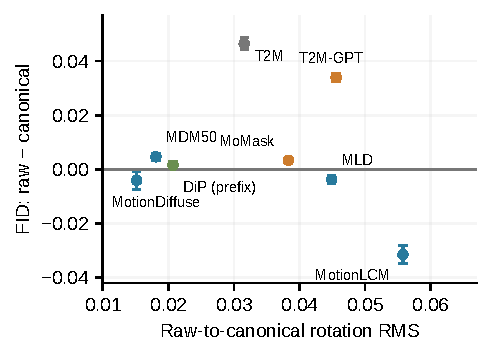
\includegraphics[width=\columnwidth]{figures/rotation_mechanism.pdf}
\caption{\textbf{Gap versus distance from canonical rotations} for the eight HumanML3D releases, with paired intervals. Blue: diffusion/consistency; orange: VQ; gray: VAE; green: prefix-conditioned.}\label{fig:mechanism}\end{figure}

\paragraph{Essential-feature readers.} The public MARDM~\cite{mardm2025} GRU and contrastive readers, which read only the 67 root and position features, are exactly invariant to rotation recoding. Their release rankings differ from that of canonical T2M by two adjacent swaps each (Kendall $\tau=0.857$ for both).

\paragraph{Published margins.} Table~1 of the main paper compares gaps with author-reported 95\% margins. These margins describe different protocols and are used only for scale. We use MDM's corrected 0.489$\pm$0.047, T2M with estimated lengths, MoMask's final KIT table and MotionDiffuse's release preprint.

\section{Attack protocols}\label{sec:attacks}
\paragraph{Targeted recoding.} We sample 1,024 full-caption test clips (40--199 frames) once, with fixed captions and crops, and use them for real motion, MDM outputs and both evaluators. Per-frame, per-joint coefficients start at zero and are optimized for 80 Adam steps (learning rate 0.1, bound 0.35) to minimize embedding distance to the actual or a circularly shifted caption, with evaluator weights frozen. R-Precision averages five fixed 32-candidate permutations. Optimizing through a canonicalizing evaluator leaves every score at its baseline. The main paper uses the T2M checkpoint released with T2M-GPT, whose real-motion scores match the published ones; \cref{tab:targeted} repeats the attack with the checkpoint distributed with MDM. Attacks against one checkpoint largely do not transfer to the other (MDM outputs attacked on the MDM-distributed checkpoint reach only 0.512 on the other), as expected for a per-clip attack with gradient access. FID moves in different directions for the two checkpoints, so the attack moves retrieval specifically rather than every metric.

\begin{table}[t]\centering\footnotesize\setlength{\tabcolsep}{3.5pt}
\setlength{\tabcolsep}{2.8pt}\caption{\textbf{Caption-targeted recoding with both T2M checkpoints}, 1,024 test clips. R1: top-1 R-Precision for the true caption, and for another clip's caption (\emph{other}). FID against the same real test clips. Real-motion R1 is 0.517 (T2M-GPT checkpoint) and 0.462 (MDM checkpoint); the published value is 0.511.}\label{tab:targeted}
\begin{tabular}{@{}llrrrr@{}}\toprule
Checkpoint&Motion&R1 before&R1 after&R1 other&FID before$\to$after\\\midrule
T2M-GPT&MDM&0.457&0.997&0.916&0.497$\to$0.393\\
T2M-GPT&Real&0.517&0.998&0.952&0.000$\to$0.385\\
MDM&MDM&0.397&0.993&0.788&0.369$\to$1.287\\
MDM&Real&0.462&0.996&0.839&0.000$\to$1.311\\
\bottomrule\end{tabular}\end{table}

\paragraph{Caption-blind recoding.} For 960 fresh MDM outputs whose source clips are disjoint from the targeted study, we compute embedding moments $(\mu_s,\Sigma_s)$ and those of 2,048 training motions $(\mu_t,\Sigma_t)$, and set per-clip targets $\mu_t+(e_i-\mu_s)T$ with the Gaussian transport map~\cite{bhatia2017}
\begin{equation}
T=\Sigma_s^{-1/2}\bigl(\Sigma_s^{1/2}\Sigma_t\Sigma_s^{1/2}\bigr)^{1/2}\Sigma_s^{-1/2},
\end{equation}
with eigenvalues floored at $10^{-4}\operatorname{tr}(\Sigma)/512$. Coefficients minimize squared distance to these targets for 80 Adam steps. No caption content, test reference or test-time score enters the optimization, and all outputs are saved before reference scoring. Two bounds, 0.1 and 0.35, were fixed in advance; the larger raises FID in every cohort (\cref{tab:blind}).

\begin{table}[t]\centering\footnotesize\setlength{\tabcolsep}{3.5pt}
\caption{\textbf{Caption-blind FID}, 960 outputs per cohort. \emph{Source}: evaluator whose gradients were used; \emph{other}: the second official T2M checkpoint, which supplied no gradients. Canonical-gradient controls stay at the original value.}\label{tab:blind}
\begin{tabular}{@{}llrrr@{}}\toprule
Cohort&Evaluator&Original&$b=0.1$&$b=0.35$\\\midrule
MDM seed 42&source&0.384&0.210&1.085\\
&other&0.408&0.334&0.972\\
MDM seed 4242&source&0.376&0.176&1.148\\
&other&0.371&0.303&0.856\\
MDM seed 7777&source&0.327&0.199&1.429\\
&other&0.379&0.284&0.779\\
MLD&source&0.706&0.289&1.611\\
&other&0.659&0.579&1.345\\
\bottomrule\end{tabular}\end{table}

\paragraph{Query-only recoding.} The attacker receives one scalar per query: the FID of its recoded outputs against the 2,048 training-motion embeddings of the primary evaluator. It sees no gradients, per-clip embeddings, captions or test reference. A (1+1) evolution strategy starts at the identity, proposes Gaussian steps of initial size $0.3b$ (multiplied by 1.5 after a success and 0.9 after a failure) and keeps a proposal only if it lowers the queried FID. It searches either 3 global coefficients or 3 coefficients per joint (63), shared across frames and clips. The best coefficients after a given number of queries are then scored once against the withheld test reference, with the primary evaluator and with the second official checkpoint, which the attacker never queried. Positions, velocities and contacts are bitwise unchanged, and canonical embeddings change by less than $10^{-6}$.

\begin{table*}[t]\centering\footnotesize\setlength{\tabcolsep}{3pt}
\caption{\textbf{Query-only recoding}, test FID after 300 queries (relative change from the original). \emph{Queried}: the evaluator that answered the queries; \emph{other}: the second checkpoint, never queried. \emph{Random}: mean of ten random coefficient vectors of the same bound on the queried evaluator.}\label{tab:blackbox}
\begin{tabular}{@{}llrrrr@{}}\toprule
Search&&MDM 42&MDM 4242&MDM 7777&MLD\\\midrule
\multicolumn{6}{@{}l}{\emph{Original FID (queried / other)}: 0.384 / 0.408, 0.376 / 0.371, 0.327 / 0.379, 0.706 / 0.659}\\
Per joint, $b=0.1$&queried&$-20\%$&$-27\%$&$-11\%$&$-57\%$\\
&other&$-30\%$&$-4\%$&$-22\%$&$-41\%$\\
&random&$+2\%$&$+3\%$&$+4\%$&$+4\%$\\
Per joint, $b=0.35$&queried&$-29\%$&$-44\%$&$-30\%$&$-68\%$\\
&other&$+51\%$&$+12\%$&$+57\%$&$+76\%$\\
&random&$+89\%$&$+74\%$&$+97\%$&$+64\%$\\
Global, $b=0.1$&queried&$-9\%$&$-11\%$&$-3\%$&$-30\%$\\
&other&$+47\%$&$+31\%$&$+28\%$&$-18\%$\\
\bottomrule\end{tabular}\end{table*}

With per-joint coefficients and $b=0.1$, the queried FID falls in every cohort and the fall carries over to the unqueried checkpoint in every cohort (\cref{tab:blackbox}). Most of the gain is reached within 100 queries. The larger bound lowers the queried FID further but overshoots for the other checkpoint, as in the gradient-based caption-blind attack. Three global coefficients are much weaker. R-Precision stays within 0.41--0.44 throughout.

\section{Reward fine-tuning}\label{sec:reward}
We fine-tune two generators against a T2M checkpoint and ask whether they move along the redundant coordinates, and we audit one reward-fine-tuned model released by others. Test inference was run only after every setting had been fixed on validation; the dated protocol, including its amendments, is released with the code.

\subsection{MDM}
\paragraph{Training.} We fine-tune the released MDM~\cite{tevet2023} (50 sampling steps, classifier-free guidance 2.5) on the 22,414 HumanML3D training clips with whole-motion captions, batch 32, AdamW (learning rate $10^{-5}$, weight decay $10^{-4}$), gradient clipping at 1 and 2,000 steps; the CLIP text encoder stays frozen. Each step has up to three terms. (i)~The usual diffusion $x_0$ loss on real training motion, computed after canonicalizing the prediction. (ii)~The reward, following ReFL~\cite{xu2023imagereward} and DRaFT~\cite{draft2024}: the model samples motions for the batch captions without gradients down to a random step $t_k\in\{0,\dots,10\}$, predicts $x_0$ at $t_k$ with gradients, and a frozen T2M checkpoint embeds this prediction, raw or canonicalized depending on the version. The loss is a symmetric InfoNCE over negative Euclidean distances between motion and text embeddings (temperature 1, weight 1), matching how R-Precision ranks captions. (iii)~A proximity penalty~\cite{fan2023dpok}: the mean squared difference, in normalized units, between the canonicalized $x_0$ predictions of the fine-tuned and the frozen pretrained model at the same noisy input (weight 100). The control uses term (i) only. Terms (i) and (iii) compare canonical motion, so the redundant coordinates receive gradient only from a raw reward.

\paragraph{Selection.} Settings were chosen on 512 validation clips with a criterion fixed in advance: raw R-Precision of the reward evaluator must rise by at least 0.03 while its raw FID stays within 1.5 times the starting value. Without the proximity penalty (diffusion loss on raw or on canonical features, learning rate $10^{-5}$ or $3\times10^{-6}$) or with penalty weight 10, reward training raised R-Precision to 0.49--0.58 but failed the FID criterion in every run (one seed each), so the weight was set to 100. At that weight the canonical-reward version qualified (R-Precision 0.420 to 0.477, raw FID 0.416 to 0.285); the raw-reward version exceeded the FID limit only when scored raw (0.660 against a limit of 0.62, canonicalized 0.244), which is the effect under study, so the setting was kept for both. Without the penalty the models moved far from the pretrained one, and every reward run drifted from canonical (off-canonical 0.036--0.065), whichever input the reward read; the penalty prevents this for canonical reward but not for raw reward. In each of the four matched pairs of these earlier runs, the raw-reward version had the larger raw-minus-canonical FID gap (0.31--0.93 against $-0.12$--0.07). The final protocol, three versions $\times$ three seeds scored once on test with final checkpoints, was fixed before any test inference; the dated protocol is released with the code. The replication with the T2M-GPT checkpoint as reward was then fixed, again before training, with no setting retuned; the no-reward control does not involve an evaluator and is shared.

\paragraph{Test scoring.} 2,048 HumanML3D test clips with one caption each, a fixed generation seed and the real test motions as FID reference. R-Precision averages five fixed 32-candidate orders. Intervals use 2,000 paired bootstrap resamples of clips, shared between raw and canonical scoring and averaged over seeds; they do not include seed-to-seed variation, which \cref{tab:rewardseeds} shows directly. \emph{Off-canonical} is the RMS difference, over valid frames, between the raw 6D rotation channels and their canonical form.

\begin{table*}[t]\centering\footnotesize\setlength{\tabcolsep}{4pt}
\caption{\textbf{Reward fine-tuning, every seed}, 2,048 test captions. Columns give scores by the MDM-distributed and the T2M-GPT-distributed T2M checkpoints. Rows marked MDM or T2M-GPT name the checkpoint that gave the reward; the other one played no part in training.}\label{tab:rewardseeds}
\begin{tabular}{@{}llrrrrrrrr@{}}\toprule
&&&\multicolumn{4}{c}{MDM checkpoint}&\multicolumn{3}{c}{T2M-GPT checkpoint}\\
\cmidrule(lr){4-7}\cmidrule(l){8-10}
Model&Seed&Off-canonical&Raw R1&$\C$ R1&Raw FID&$\C$ FID&Raw R1&Raw FID&$\C$ FID\\\midrule
Pretrained&--&0.019&0.415&0.418&0.332&0.327&0.463&0.401&0.400\\
No reward&42&0.019&0.424&0.423&0.395&0.391&0.480&0.450&0.439\\
No reward&123&0.019&0.430&0.429&0.398&0.397&0.478&0.470&0.464\\
No reward&777&0.018&0.427&0.427&0.467&0.464&0.479&0.489&0.481\\\midrule
Canonical reward, MDM&42&0.019&0.490&0.491&0.223&0.261&0.491&0.295&0.286\\
Canonical reward, MDM&123&0.019&0.491&0.491&0.173&0.211&0.494&0.303&0.296\\
Canonical reward, MDM&777&0.019&0.488&0.489&0.308&0.364&0.487&0.388&0.379\\
Raw reward, MDM&42&0.042&0.491&0.491&0.775&0.283&0.488&0.409&0.365\\
Raw reward, MDM&123&0.043&0.500&0.488&0.656&0.258&0.484&0.416&0.379\\
Raw reward, MDM&777&0.046&0.496&0.484&0.823&0.312&0.482&0.488&0.464\\\midrule
Canonical reward, T2M-GPT&42&0.018&0.448&0.448&0.280&0.275&0.533&0.151&0.154\\
Canonical reward, T2M-GPT&123&0.019&0.453&0.453&0.255&0.252&0.532&0.167&0.172\\
Canonical reward, T2M-GPT&777&0.018&0.448&0.448&0.304&0.299&0.527&0.180&0.184\\
Raw reward, T2M-GPT&42&0.040&0.448&0.446&0.290&0.333&0.531&0.264&0.211\\
Raw reward, T2M-GPT&123&0.040&0.451&0.450&0.240&0.292&0.535&0.262&0.277\\
Raw reward, T2M-GPT&777&0.039&0.445&0.442&0.339&0.397&0.540&0.206&0.338\\
\bottomrule\end{tabular}\end{table*}

\paragraph{Results.} On validation, the off-canonical distance of every raw-reward run grows steadily, from 0.020 at the start to 0.040--0.046 after 2,000 steps, while the control and canonical-reward runs stay at 0.018--0.019. The test gaps below are raw minus canonical, by the checkpoint named.

\emph{MDM checkpoint as reward.} Raw reward: FID $+0.467$ [0.278, 0.658] and R1 $+0.008$ [0.002, 0.014] by the reward checkpoint; FID $+0.035$ [$-0.035$, 0.109] and R1 $+0.002$ [$-0.002$, 0.006] by the other. Canonical reward: FID $-0.044$ [$-0.076$, $-0.015$] and R1 $-0.001$ [$-0.002$, 0.001] by the reward checkpoint. Control: FID $+0.003$ [0.001, 0.005] and R1 $+0.001$ [$-0.000$, 0.002].

\emph{T2M-GPT checkpoint as reward.} Raw reward: FID $-0.031$ [$-0.118$, 0.058] and R1 $+0.009$ [0.002, 0.016] by the reward checkpoint; FID $-0.051$ [$-0.074$, $-0.027$] and R1 $+0.002$ [$-0.000$, 0.005] by the other. Canonical reward: FID $-0.004$ [$-0.007$, $-0.001$] and R1 $+0.001$ [$-0.000$, 0.002] by the reward checkpoint. Control, by this checkpoint: FID $+0.008$ [0.004, 0.013] and R1 $+0.002$ [0.001, 0.003].

\paragraph{Reading the two checkpoints together.} Three findings hold with both rewards: raw reward, and only raw reward, drives the outputs off canonical; it raises the reward checkpoint's R-Precision through the encoding by about 0.01; and it moves FID by more than the control's gap with at least one checkpoint. Size and sign of the FID change differ. With MDM's checkpoint as reward its own FID rises sharply; with T2M-GPT's as reward its own FID gap varies in sign across seeds ($+0.053$, $-0.015$, $-0.132$), while MDM's checkpoint, as judge, consistently rates the raw outputs better than their canonical form. The comparison between the two reward versions under that judge (raw scores level, canonical scores separating them in every seed) was not a planned endpoint and is reported as an observation. Like released generators (\cref{sec:natural}), canonical-reward models keep small nonzero gaps.

The checkpoint that gave no reward is also less impressed by the fine-tuning itself. After canonicalization it rates canonical-reward models better than the pretrained model (FID 0.32 against 0.40, and 0.28 against 0.33), but raw-reward models no better (0.40 against 0.40, and 0.34 against 0.33); their R-Precision gains over the control are smaller than for the reward checkpoint (0.479 to 0.48--0.49, and 0.427 to 0.45). Raw reward may therefore cost some real quality as well. These are the familiar differences between a proxy reward and an independent judge~\cite{gao2023overoptimization}; the encoding result concerns the raw-minus-canonical gaps of the same outputs and does not depend on them.

\subsection{A second generator: MLD}
\paragraph{Training.} MLD~\cite{mld2023} denoises a 256-dimensional latent that a frozen VAE decodes into HumanML3D features. We fine-tune only the denoiser of the released checkpoint with the same reward as for MDM (MDM's checkpoint, the same InfoNCE loss and weight, reward at a random step among the last 11 of 50), its native DDIM-50 sampler with guidance 7.5, learning rate $10^{-5}$, batch 32 and 2,000 steps. Unlike for MDM, both regularizers are MLD's own latent-space terms, which do not single out the redundant coordinates: the noise-prediction loss on VAE latents of real training motion (10\% caption dropout), and a penalty on the squared difference between the guided noise predictions of the fine-tuned and frozen denoisers at the reward step.

\paragraph{Selection.} The criterion was the one used for MDM. Penalty weights 10, 100 and 1,000 left the reward almost inactive (R-Precision gain at most 0.019 on validation), so none qualified; the grid was then extended to 1 and 0, before any MLD test inference. The fixed rule, the smallest weight at which the canonical-reward version qualifies, selected 0, so unlike MDM the confirmed MLD runs have no proximity penalty. Weight 1, which also qualified, shows the same picture on validation: off-canonical 0.051 (raw reward) and 0.050 (canonical reward), FID gaps $-0.009$ and $-0.005$. Three versions $\times$ three seeds were scored once on the same 2,048 test clips as MDM.

\begin{table*}[t]\centering\footnotesize\setlength{\tabcolsep}{5pt}
\caption{\textbf{Reward fine-tuning of MLD}, 2,048 test captions, mean of three seeds. R1 and FID by MDM's checkpoint, which gave the reward; the last two columns by the T2M-GPT checkpoint.}\label{tab:rewardmld}
\begin{tabular}{@{}lrrrrrrr@{}}\toprule
&&\multicolumn{4}{c}{MDM checkpoint (reward)}&\multicolumn{2}{c}{T2M-GPT checkpoint}\\
\cmidrule(lr){3-6}\cmidrule(l){7-8}
Model&Off-canonical&Raw R1&$\C$ R1&Raw FID&$\C$ FID&Raw FID&$\C$ FID\\\midrule
Pretrained&0.044&0.441&0.441&0.489&0.508&0.367&0.377\\
No reward&0.043&0.437&0.438&0.767&0.788&0.520&0.533\\
Canonical reward&0.060&0.555&0.554&0.235&0.202&0.329&0.279\\
Raw reward&0.061&0.554&0.551&0.199&0.169&0.292&0.247\\
\bottomrule\end{tabular}\end{table*}

\paragraph{Results.} \Cref{tab:rewardmld}. Both reward versions raise R-Precision equally (from 0.441 to 0.554 and 0.555) and move off canonical form equally (0.061 and 0.060, against 0.044 for the pretrained model and 0.043 for the control). The raw-minus-canonical FID gap by the reward checkpoint changes sign in both: $-0.019$ [$-0.030$, $-0.010$] for the pretrained model and $-0.021$ [$-0.030$, $-0.012$] for the control, against $+0.031$ [0.011, 0.051] for raw and $+0.033$ [0.014, 0.053] for canonical reward; by the other checkpoint, $+0.045$ [0.022, 0.069] and $+0.050$ [0.028, 0.073]. The R-Precision gap of the reward checkpoint is $+0.003$ [0.000, 0.006] for raw and $+0.001$ [$-0.002$, 0.003] for canonical reward. Unlike MDM, MLD shows no meaningful difference between the two reward inputs: fine-tuning moves its outputs along the redundant coordinates whichever input the reward reads, and the encoding then changes its FID in either case. One possible reason is that MLD reaches the features only through a decoder trained on canonical motion and kept frozen; we did not test this. The absence of a difference is not explained by the missing penalty alone, since validation at weight 1 (one seed) shows it too.

\subsection{A released reward-fine-tuned model}
 MotionRFT~\cite{motionrft2026} releases an MLD~\cite{mld2023} fine-tuned with the authors' own learned reward, together with the base checkpoint it starts from. We generated five native cohorts of 1,024 outputs with each (captions and lengths of the first five MDM audit draws, generation seeds 2101--2105, the native DDIM-50 sampler with guidance 7.5) and scored raw and canonicalized outputs with both T2M checkpoints against the native test reference, with paired $t_4$ intervals Bonferroni-adjusted over eight endpoints. The off-canonical distance is 0.044--0.046 for the base model and 0.049--0.051 for the fine-tuned one, higher in every cohort. Raw-minus-canonical FID is $-0.016$ [$-0.039$, 0.007] (MDM checkpoint) and $-0.003$ [$-0.010$, 0.004] (T2M-GPT checkpoint) for the base model, and $+0.036$ [0.028, 0.045] and $+0.028$ [0.008, 0.048] for the fine-tuned model; R-Precision gaps include zero for both. The MLD study above shows the same pattern, a drift off canonical form and an FID gap that turns positive, whether the reward reads raw or canonical input, so we do not attribute it to the authors' reward reading rotations. What it does show is that fine-tuning changed how much this model's score depends on the encoding, a change that canonical evaluation removes.

\section{Sign language}\label{sec:sign}
\paragraph{Data and readers.} We use the released SignSparK body and hand rotation features~\cite{low2026} (240 per frame: 10 body and $2\times15$ hand joints) and the public backtranslation readers~\cite{signsparkbt}, one Sign Language Transformer~\cite{camgoz2020} per corpus, with native tokenization, beam search and 300-frame cap. Full test sets contain 642 PHOENIX-2014T~\cite{camgoz2018}, 2,183 How2Sign~\cite{duarte2021} and 1,162 CSL-Daily~\cite{zhou2021} clips; real-motion BLEU is 15.00, 3.48 and 6.89. Left-hand channels, which the released pipeline preprocesses canonically, are unchanged in every attack.

\subsection{Real-input stability controls}\label{sec:signstability}
We decode the same full How2Sign and CSL-Daily test inputs under canonicalization, Gaussian noise and physical rotation changes, keeping input order, crops, reader weights, vocabularies and beam settings fixed. Every path shares native preprocessing. The reader receives only motion and valid lengths; captions are used only after decoding to compute BLEU. Canonicalization changes 1,438 How2Sign and 464 CSL-Daily hypotheses, while all 642 PHOENIX hypotheses remain unchanged.

\paragraph{Matched input norms.} Each clip uses its actual canonicalization displacement $B=\|\C(x)-x\|_2$ over valid frames. Three fixed Gaussian fields on body/right-hand channels are individually rescaled to $B$, preserving the preprocessed left-hand stream. Their per-clip average is the primary Gaussian control; a secondary field perturbs all 240 channels. No field uses captions or evaluator gradients.

Physical controls rotate both original three-vectors together about a per-joint isotropic axis fixed through time. This changes represented rotations while preserving the vectors' norms and inner product; the left hand remains fixed. The matched control solves a per-clip angle to reach the same $B$: mean angles are $2.623^\circ$ on How2Sign and $5.293^\circ$ on CSL-Daily, with maxima $5.470^\circ$ and $9.756^\circ$. A separate one-degree control has a different input norm. Realized matched-norm errors divided by $\max(B,1)$ are below $5\times10^{-8}$.

\begin{table*}[t]
\centering\small
\caption{\textbf{Every real-sign stability condition.} Same full native test clips and frozen decoder. Changed hypotheses use words on How2Sign and characters on CSL; normalized edit distance (NED) divides Levenshtein distance by the larger output length, with minimum one. Each Gaussian field and all BLEUs are retained. Same-support noise and physical controls protect the preprocessed left hand.}\label{tab:signstabilityall}
\begin{tabular}{@{}llrrrr@{}}\toprule
Corpus&Condition&Changed \%&Mean edits&NED&BLEU\\\midrule
How2Sign&Raw&0.0&0.000&0.000&3.4779\\
How2Sign&Canonical&65.9&8.121&0.397&3.4840\\
How2Sign&Gaussian support 1&41.2&5.002&0.243&3.5053\\
How2Sign&Gaussian support 2&43.0&5.169&0.251&3.5494\\
How2Sign&Gaussian support 3&41.5&4.812&0.235&3.4852\\
How2Sign&Gaussian all240&37.2&4.556&0.220&3.5763\\
How2Sign&Physical $1^\circ$&45.4&5.208&0.252&3.6018\\
How2Sign&Physical matched&70.3&8.634&0.426&3.5538\\
CSL&Raw&0.0&0.000&0.000&6.8907\\
CSL&Canonical&39.9&5.167&0.304&7.0662\\
CSL&Gaussian support 1&22.9&2.984&0.173&6.8595\\
CSL&Gaussian support 2&21.7&2.855&0.165&6.6456\\
CSL&Gaussian support 3&22.5&2.916&0.167&6.7068\\
CSL&Gaussian all240&20.5&2.678&0.156&6.9470\\
CSL&Physical $1^\circ$&13.9&1.757&0.102&7.0123\\
CSL&Physical matched&44.3&5.923&0.346&6.5762\\
\bottomrule\end{tabular}\end{table*}

\begin{table*}[t]
\centering\small
\caption{\textbf{Primary paired stability intervals.} Twenty-endpoint-adjusted intervals, 20,000 cluster bootstraps; official VIDEO\_ID on How2Sign, clip on CSL. The Gaussian support mean averages the three fixed fields per clip. Intervals condition on these test inputs, reader weights and noise fields; they do not estimate model-training uncertainty.}\label{tab:signstabilityintervals}
\begin{tabular}{@{}llrrrr@{}}\toprule
Corpus&Condition&Changed \%&95\% interval&NED&95\% interval\\\midrule
How2Sign&Canonical&65.9&$[61.7,69.8]$&0.397&$[0.366,0.429]$\\
How2Sign&Gaussian support mean&41.9&$[38.9,45.0]$&0.243&$[0.223,0.264]$\\
How2Sign&Gaussian all240&37.2&$[33.8,40.8]$&0.220&$[0.197,0.244]$\\
How2Sign&Physical $1^\circ$&45.4&$[41.9,49.1]$&0.252&$[0.228,0.278]$\\
How2Sign&Physical matched&70.3&$[66.6,74.1]$&0.426&$[0.396,0.458]$\\
CSL&Canonical&39.9&$[35.5,44.2]$&0.304&$[0.269,0.339]$\\
CSL&Gaussian support mean&22.3&$[19.6,25.2]$&0.168&$[0.147,0.191]$\\
CSL&Gaussian all240&20.5&$[17.0,24.2]$&0.156&$[0.128,0.186]$\\
CSL&Physical $1^\circ$&13.9&$[10.8,17.0]$&0.102&$[0.078,0.125]$\\
CSL&Physical matched&44.3&$[40.0,48.7]$&0.346&$[0.312,0.382]$\\
\bottomrule\end{tabular}\end{table*}

\begin{table*}[t]
\centering\small
\caption{\textbf{Canonicalization minus matched controls.} Separate eight-endpoint-adjusted paired contrasts. Positive changes indicate a larger decoding change from canonicalization; negative changes indicate a larger change from the control. Neither sign establishes semantic accuracy or that physical changes are linguistically irrelevant.}\label{tab:signstabilitycontrasts}
\begin{tabular}{@{}llrrrr@{}}\toprule
Corpus&Control&$\Delta$ changed (pp)&95\% interval&$\Delta$ NED&95\% interval\\\midrule
How2Sign&Gaussian support mean&+24.0&$[+21.0,+26.7]$&+0.154&$[+0.133,+0.174]$\\
How2Sign&Physical matched&-4.4&$[-7.6,-1.3]$&-0.030&$[-0.053,-0.006]$\\
CSL&Gaussian support mean&+17.6&$[+13.9,+21.4]$&+0.136&$[+0.106,+0.167]$\\
CSL&Physical matched&-4.4&$[-9.0,+0.2]$&-0.042&$[-0.080,-0.005]$\\
\bottomrule\end{tabular}\end{table*}


\paragraph{Measurements and uncertainty.} Changed hypotheses compare decoded strings; edit distance uses words on How2Sign and characters with punctuation on CSL-Daily, without reference captions. Normalized edit distance (NED) divides Levenshtein distance by the larger output length, with minimum one; empty outputs remain included. Twenty thousand paired cluster bootstraps resample the 149 official How2Sign video identifiers or CSL-Daily clips, sharing resampling weights across conditions. Primary intervals adjust twenty endpoints (five summarized conditions, two corpora, two measures); canonical-minus-control contrasts adjust a separate eight-endpoint family. These intervals condition on the readers, test inputs and three noise fields rather than estimating model-training uncertainty.

\paragraph{Results.} Canonicalization changes more hypotheses and yields larger NED than same-support Gaussian noise in both corpora; all four adjusted paired contrasts exclude zero. Matched physical changes have larger mean effects. Both How2Sign physical contrasts exclude zero; CSL-Daily's changed-fraction contrast includes zero, while its NED contrast does not. The controls establish encoding sensitivity relative to the tested Gaussian fields, alongside sensitivity to physical changes. They do not imply improved semantic accuracy or that small physical changes are linguistically irrelevant. \Cref{tab:signstabilityall,tab:signstabilityintervals,tab:signstabilitycontrasts} report every condition, the primary intervals and the paired contrasts.

\subsection{Learned and per-clip recodings}
\paragraph{Learned layers.} The PHOENIX layer (299k parameters) reads a frozen text-to-motion diffusion model's output and the source sentence, encoded by the generator's frozen text encoder, and predicts bounded coefficients with cross-attention and three dilated temporal convolutions. It is trained for 20 epochs on 7,096 training motions with the reader's caption cross-entropy; generator and reader are frozen and final checkpoints are used. The How2Sign and CSL-Daily layers (770k parameters) read real training motion and the reader's own word embeddings. \Cref{tab:layers} reports ablations: without the source sentence the gain is small, and with the loss computed after canonicalization it vanishes, as Eq.~(4) of the main paper predicts.

\begin{table}[t]\centering\footnotesize\setlength{\tabcolsep}{3.5pt}
\caption{\textbf{Learned-layer ablations}, full test sets. Raw BLEU and gain over no layer with paired 95\% intervals; canonical hypotheses are unchanged in every row. How2Sign/CSL controls use one seed.}\label{tab:layers}
\begin{tabular}{@{}llrr@{}}\toprule
Corpus&Layer input / loss&Raw&Gain [95\% CI]\\\midrule
PHOENIX&text+motion / raw&15.21&8.81 [7.82, 9.87]\\
&motion only / raw&7.60&1.21 [0.66, 1.76]\\
&text+motion / canonical&6.26&$-0.13$ [$-0.32$, 0.04]\\
How2Sign&text+motion / raw&6.11&2.64 [2.27, 3.03]\\
&text+motion / canonical&3.48&0.00 [$-0.18$, 0.20]\\
CSL-Daily&text+motion / raw&7.43&0.54 [0.14, 0.97]\\
&text+motion / canonical&6.79&$-0.10$ [$-0.40$, 0.09]\\
\bottomrule\end{tabular}\end{table}

\paragraph{Per-clip attacks.} On 128 real test clips per corpus, 80 Adam steps toward a circularly shifted sentence raise BLEU against that sentence to 85.19 (PHOENIX), 47.34 (How2Sign) and 32.44 (CSL-Daily), while BLEU against the actual sentence drops to 0.00, 0.00 and 1.26; canonical hypotheses are unchanged. A gloss-level CTC recognizer of a different architecture shows the same failure (wrong-target WER 118\%$\to$4\%).

\paragraph{Detector statistics.} Write $s=(\rho-1,\sigma-1,\tau)$. The squared distance to the canonical encoding is $E=\|s\|^2$, and the squared feature norm satisfies $N-E=2(\rho+\sigma)-2$, so rotating $s$ about $(1,1,0)/\sqrt2$ preserves both. A per-clip attack restricted to this circle (200 steps) raises PHOENIX BLEU from 6.62 to 10.72 (+4.09, 95\% CI [3.04, 5.24]), while a threshold detector on the RMS distance to canonical has AUC 0.500. Fixing the full $2\times2$ Gram matrix of $(a,b)$ would leave no channel; matching a few statistics is therefore not a general defense, whereas canonicalization closes the whole fiber.

\paragraph{Reader adaptation.} Real How2Sign and CSL-Daily features are not canonical. We fine-tune each public reader for five epochs on raw or on canonical training features, with three seeds each and matched batches. Test BLEU is 3.37 raw versus 3.47 canonical on How2Sign (difference $+0.10$, 95\% CI [$-0.01$, 0.21]) and 7.24 versus 7.22 on CSL-Daily ($-0.02$, [$-0.19$, 0.15]). Canonical readers keep every hypothesis under fresh attacks and under fixed equivalent recodings of all 10,035 test inputs.

\section{Statistics and reproducibility}\label{sec:stats}
Motion audits use paired $t_{19}$ intervals over 20 native draws, Bonferroni-adjusted within each stated family. Sign-language intervals use 20,000 paired bootstrap resamples that recompute corpus BLEU from sufficient statistics, clustered by the 149 official How2Sign video identifiers; seed sensitivity additionally resamples the three fitting seeds. Corpus BLEU and WER are recomputed with independent implementations. Clip selections, seeds and bounds were fixed before scoring, and no checkpoint was selected on test scores. Experiments ran with PyTorch 2.11 and CUDA 12.8 on one RTX PRO 6000; exact floating-point decoding can depend on hardware.

\clearpage
{\small\bibliographystyle{ieeenat_fullname_citation}\bibliography{references}}
\end{document}
